%!TEX root = ../ltransform.tex
\section{Метод обращения волнового фронта излучения}

Одной из важнейших задач квантовой электроники является уменьшение угловой расходимости лазерного излучения, достижение минимальной дифракционной расходимости
\begin{equation}
	\Delta \theta = \frac{\lambda}{D},
\end{equation}
где $\Delta \theta$ - угловая ширина диаграммы направленности, $\lambda$ - длина волны и $D$ - характерный размер области источника излучения. Главная причина, по которой расходимость генерируемых лазерами полей превосходит дифракционную, состоит в том, что в оптических трактах лазерных устройств обычно присутствуют всевозможные неоднородности диэлектрической проницаемости, вносящие негативный вклад в структуру фазового фронта распространяющегося излучения. Поскольку техническое устранение даже небольшой части неоднородностей является крайне сложным, то чрезвычайно актуальными представляются исследования и разработки новых методов передачи энергии и информации в оптике, позволяющих обеспечить высокие выходные характеристики лазерного излучения. В литературе они получили наименование методов фазовой коррекции волновых фронтов излучения.

В настоящем параграфе мы обсудим одно замечательное явление нелинейной оптики, которое может быть использовано для устранения негативного влияния оптических неоднородностей на структуру распространяющихся электромагнитных полей. Это явление называется эффектом обращения волнового фронта (ОВФ) излучения.

\begin{figure}[ht]
	\centering
	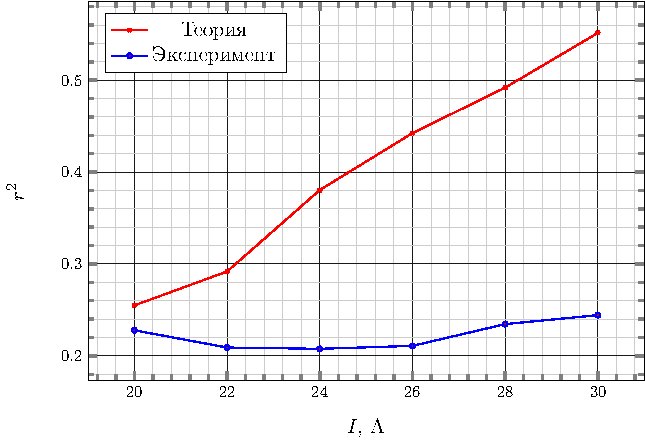
\includegraphics[scale=1.5]{fig/fig2.pdf}
	\caption{}
	\label{fig:figure2}
\end{figure}

Прежде всего, поясним идею эффекта ОВФ и метода коррекции, на нём основанного. Пусть на фотопластинку ГФ (Рис. \ref{fig:figure2}) падает волна сигнала $\vec{E}_3$ и когерентная с ней опорная волна $\vec{E}_1$. Картина интерференции полей записывается в фотослое. Фотопластинка обрабатывается так, что интерференционные неоднородности проявляются в виде модуляции её прозрачности для излучения на частоте, на которой была создана и записана интерференционная картина. Получается так называемая голограмма. Если она достаточно тонкая, то ее действие на восстанавливающую волну можно описать введением комплексного коэффициента пропускания $\tilde{\Pi}$ для амплитуды поля
\begin{equation}
	\label{eq:2.1}
\tilde{E}_{\tau}(\vec{r}\,)=\tilde{\Pi}(\vec{r}\,) \tilde{E}_{i}(\vec{r}\,),
\end{equation}
где $ \tilde{E}_{i}$  падающее на слой и $ \tilde{E}_{\tau}$ - прошедшее через слой поля.

В простейшем случае вариации $R$ связаны с изменениями интенсивности записываемого поля, так что голограмма-транспарант имеет прозрачность
\begin{equation}
	\label{eq:2.2}
	\tilde{\Pi}(\vec{r}\,)=\operatorname{const}_{0} \cdot\left\{\tilde{E}_{1} \tilde{E}_{3}^{*}+\text {к.c.}\right\} \equiv C_{0} \cdot\left\{\tilde{E}_{1} \tilde{E}_{3}^{*}+\text {к.c.}\right\}
\end{equation}
Если направлять на транспарант считывающую волну $\vec{\tilde{E}}_2$ так,
 чтобы она распространялась точно навстречу опорной волне ($\tilde{E}_2 \sim \tilde{E}_1^*$), то после прохождения волны $\vec{\tilde{E}}_2$ через
  голограмму в соответствии с соотношением \eqref{eq:2.1} за счет первого слагаемого в \eqref{eq:2.2} восстанавливается поле
\begin{equation}
	\label{eq:2.3}
	\tilde{E}_{4}(\vec{r}\,) \sim\left|\tilde{E}_{1}(\vec{r}\,)\right|^{2} \tilde{E}_{3}^{*}(\vec{r}\,),
\end{equation}
распространяющееся навстречу сигналу $\tilde{E}_3$ и при $|\vec{\tilde{E}}_1|^2 = \mathrm{const}_1 = E_0^2$ отвечающее точно обращённой к сигналу волне.

\begin{figure}[h]
	\centering
	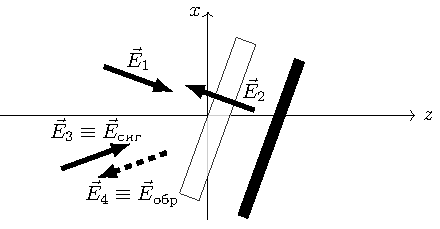
\includegraphics[scale=1.5]{fig/fig3.pdf}
	\caption{Волны $\vec{E}_{1,2}$ -- опорные, $\vec{E}_3$ -- сигнальная, $\vec{E}_4$ -- обращённая}
	\label{fig:figure3}
\end{figure}

Теперь представим себе, что для записи голограммы используется нелинейная среда (Рис. \ref{fig:figure3}) с диэлектрической проницаемостью
\begin{equation}
	\label{eq:2.4}
	\varepsilon=\varepsilon_{0}+\delta \varepsilon
	\left(
	\overline{{|\vec{E}|^{2}}}^{(2 \pi / \omega)}
	\right).
\end{equation}
В нелинейный слой одновременно направляются две опорных плоских волны
\begin{equation}
	\label{eq:2.5}
	\vec{E}_{1.2} =\operatorname{Re}\left\{\vec{\tilde{E}}_{1,2} \exp \left[i\left(\omega t \mp k_{z} z \pm k_{x} x\right)\right]\right\}
\end{equation}
и сигнальная волна
\begin{equation}
	\label{eq:2.6}
	\vec{E}_{3} =\operatorname{Re}\left\{\vec{\tilde{E}}_{3} \exp \left[i\left(\omega t-k_{z} z-k_{x} x\right)\right]\right\}.
\end{equation}
При этом вторая опорная плоская волна получается отражением первой от зеркала. В нелинейной среде \eqref{eq:2.4} процессы записи голографической решетки $(\delta \varepsilon)_{13} \sim \vec{\tilde{E}}_{1} \vec{\tilde{E}}_{3}^{*}+\text{к.с.}$ и ее считывания $(\delta \varepsilon )_{13} \cdot \vec{E}_2$ совмещены во времени.
Это -- динамическая голография. Динамическая голограмма обращает любую падающую сигнальную волну, автоматически подстраиваясь под нее. При этом обращенная волна
\begin{equation}
	\label{eq:2.7}
	\vec{\tilde{E}}_4 \sim \vec{\tilde{E}}_3^*
\end{equation}
возбуждается практически мгновенно, т.е. в реальном масштабе времени. Динамическую голограмму, обращающую волновой фронт падающего на нее излучения, называют ОВФ-зеркалом. Не трудно понять, как с помощью такого ОВФ-зеркала можно создать оптическую систему, способную скомпенсировать искажения сигнала (изображения) из-за наличия неоднородностей на трассе оптического пути внутри самого принимающего устройства.

\begin{figure}[ht]
	\centering
	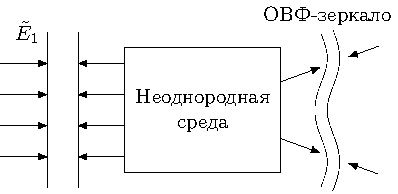
\includegraphics[scale=1.4]{fig/fig4.pdf}
	\caption{}
	\label{fig:figure4}
\end{figure}

Пусть плоская волна проходит через неоднородную среду, которая
искажает структуру её фазового фронта (Рис. \ref{fig:figure4}). На поверхность зеркала, которое должно формировать встречную волну, поступает поле
\begin{equation}
	\label{eq:2.8}
	\tilde{\Pi}(\vec{r}\,) \tilde{E}_{1} \sim \tilde{E}_{1} \exp [i \psi(\vec{r}\,)],
\end{equation}
где экспоненциальный множитель описывает влияние фазовых неоднородностей. С помощью обыкновенного зеркала можно сформировать отражённую волну, имеющую поле
\begin{equation}
	\label{eq:2.8'}
	\tilde{E}_{2} \sim \tilde{E}_{1} \exp [i \psi(\vec{r}\,)] \equiv \tilde{\Pi}(\vec{r}\,) \tilde{E}_{1}.
\end{equation}
Если рефлектором будет ОВФ-зеркало, то от него отразится поле
\begin{equation}
	\label{eq:2.9}
	\tilde{E}_{2} \sim \tilde{\Pi}^{*}(\vec{r}\,) \tilde{E}_{1}^{*} \equiv \tilde{E}_{1}^{*} \exp [-i \psi(\vec{r}\,)],
\end{equation}
которое после повторного прохождения волны через среду примет вид
\begin{equation}
	\label{eq:2.10}
	\tilde{E}_{3} \sim \tilde{E}_{2} \exp [i \psi(\vec{r}\,)] \sim \tilde{E}_{1}^{*}.
\end{equation}
\begin{figure}[hb]
	\centering
	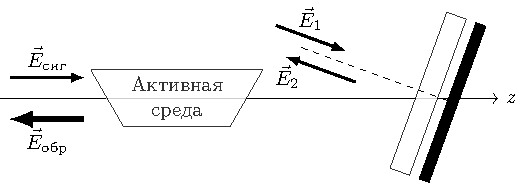
\includegraphics[scale=1.4]{fig/fig5.pdf}
	\caption{Волны $\vec{E}_{1,2}$ -- опорные, $\vec{E}_\text{сиг}\equiv\vec{E}_3$ -- сигнальная, $\vec{E}_\text{обр}\equiv\vec{E}_4$ -- обращённая}
	\label{fig:figure5}
\end{figure}
Таким образом, влияние фазовых неоднородностей будет ликвидировано. Если в качестве неоднородного материала взять активную среду, то получится двухпроходовый усилитель (Рис. \ref{fig:figure5}), фазовые неоднородности которого никак не влияют на усиливаемое излучение.





\subsection{ОВФ при четырёхволновом смешении в среде с тепловым механизмом нелинейности}

Важнейшей характеристикой ОВФ-зеркала, работающего в стационар­ном режиме, является комплексный коэффициент отражения
\begin{equation}
	\label{eq:2.11}
	\tilde{r}(0)=\frac{\tilde{\mathcal{E}}_{4}^{*}(0)}{\tilde{\mathcal{E}}_{3}(0)}.
\end{equation}
Чтобы найти эту величину для ОВФ-зеркала, выполненного на основе неподвижной ($\vec{v}_0 = 0$) проводящей ($\sigma_0$) среды с тепловым механизмом нелинейности, необходимо воспользоваться стационарными уравнениями для поля
\begin{equation}
	\label{eq:2.12}
	\Delta \tilde{E}+k^{2} \tilde{E}-i k^{2} \frac{4 \pi \sigma_{0}}{\varepsilon_{0} \omega} \tilde{E}=-k^{2} \frac{\delta \varepsilon}{\varepsilon_{0}} \tilde{E}
\end{equation}
и нелинейной диэлектрической проницаемости
\begin{equation}
	\label{eq:2.13}
	\frac{\delta \varepsilon}{\tau_{0}}-\chi \Delta \delta \varepsilon=\frac{\sigma_{0}}{\rho_{0} C_{p}} \cdot\left(\frac{\partial \varepsilon}{\partial T}\right)_{p} \overline{|\vec{E}|^{2}}^{(2\pi/\omega)}.
\end{equation}
Уравнение \eqref{eq:2.13} описывает структуру объёмных решёток $\delta \varepsilon$ индуцированных полем четырёх волн
\begin{equation}
	\label{eq:2.14}
	\begin{aligned}
	\tilde{E} &=\left[\tilde{E}_{1} \exp \left(i k_{x} x\right)+\tilde{E}_{3} \exp \left(-i k_{x} x\right)\right] \exp \left(-i k_{z} z\right)+\\
	&+\left[\tilde{E}_{2} \exp \left(-i k_{x} x\right)+\tilde{E}_{4} \exp \left(i k_{x} x\right)\right] \exp \left(i k_{z} z\right).
	\end{aligned}
\end{equation}
Две решётки записываются попутными волнами $\tilde{E}_1$, $\tilde{E}_3$, и $\tilde{E}_2$, $\tilde{E}_4$, ещё четыре - встречными. Решётки попутных и встречных волн называются со­ответственно <<пропускающими>> и <<отражающими>> решётками $\delta \varepsilon$. Вклад каждой из них в процесс ОВФ-ЧВС определяется величиной их собственного времени релаксации $\tau_\text{r}$. Время релаксации существенно зависит от геометрии записи.
При условии $1 / \tau_0 \ll \chi \cdot (2\pi / \lambda)^2$ оно пропорционально квадрату пространственного периода соответствующей решетки, и поэтому при $(k_x / k_z) = \tg\theta \approx \theta \ll 1$ собственное время релаксации <<пропускающих>> решеток в $\theta^{-2}$ раз больше времени релаксации <<отражающих>>. В типичном случае, когда $\theta \approx 10^{-2}$ рад, $\lambda \approx 1$ мкм, $\chi \approx 10^{-3}$ см${}^2$/сек, время релаксации <<пропускающих>> решеток согласно \eqref{eq:pdv.37} будет составлять $\tau_\text{rt} \approx 10^{-3}$ сек, а <<отражающих>> $\tau_\text{rr} \sim 10^{-8}$ сек. Из \eqref{eq:pdv.39} и \eqref{eq:pdv.41} следует, что соответствующие параметры нелинейности $G_\text{rt}$, $G_\text{rr}$ и пропорциональные им амплитуды решёток будут различаться по своей величине на 5 порядков. Это значит, что при расчёте коэффициента отражения стационарного ОВФ-зеркала учёт <<отражающих>> решёток может внести поправки порядка $10^{-5}$ от основного результата. Поскольку столь малого вклада в эффект ОВФ, связанного с <<отражающими>> решетками, невозможно заметить экспериментально, то решение уравнения \eqref{eq:2.13} следует искать в виде
\begin{equation}
	\label{eq:2.15}
	\delta \varepsilon(z) \cong \delta \varepsilon^{\prime \prime}(z)+\left[\frac{1}{2} \delta \tilde{\varepsilon}(z) \exp \left(2 i k_{x} x\right)+\text{к.с.}\right],
\end{equation}
где средняя составляющая $\delta \varepsilon ''(z)$ и комплексная амплитуда $\delta \tilde{\varepsilon} (z)$ решётки $\delta \varepsilon$ по координате $x$ являются медленно меняющимися на длине волны $\lambda = (2\pi / k)$ функциями координаты $z$.

Подставляя \eqref{eq:2.15} в \eqref{eq:2.13} и \eqref{eq:2.14} в \eqref{eq:2.12}, можно получить по аналогии с тем,
как были получены уравнения \eqref{eq:pdv.29} -- \eqref{eq:pdv.31}, систему связанных уравнений
\begin{equation}
	\label{eq:2.16}
	\frac{1}{\tau_{0}} \delta \varepsilon^{\prime \prime}(z) \cong \frac{\sigma_{0}}{2 \rho_{0} C_{p}}\left(\frac{\partial \varepsilon}{\partial T}\right)_{p} \cdot \sum_{q=1}^{4}\left|\tilde{E}_{\mathrm{q}}\right|^{2},
\end{equation}
\begin{equation}
	\label{eq:2.17}
	\left[\chi \cdot 4 k_{x}^{2}+\frac{1}{\tau_{0}}\right] \delta \tilde{\varepsilon}(z) \cong \frac{\sigma_{0}}{\rho_{0} C_{p}} \cdot\left(\frac{\partial \varepsilon}{\partial T}\right)_{p} \cdot\left(\tilde{E}_{1} \tilde{E}_{3}^{*}+\tilde{E}_{2}^{*} \tilde{E}_{4}\right),
\end{equation}
\begin{equation}
	\label{eq:2.18}
	-2 i k_{z} \frac{\partial E_{1}}{\partial z}-i k^{2} \frac{4 \pi \sigma_{0}}{\varepsilon_{0} \omega} \tilde{E}_{1} \cong-\frac{k^{2}}{\varepsilon_{0}}\left\{\delta \varepsilon^{\prime \prime} \cdot \tilde{E}_{1}+\frac{1}{2} \delta \tilde{\varepsilon} \cdot \tilde{E}_{3}\right\},
\end{equation}
\begin{equation}
	\label{eq:2.19}
	-2 i k_{z} \frac{\partial \tilde{E}_{3}}{\partial z}-i k^{2} \frac{4 \pi \sigma_{0}}{\varepsilon_{0} \omega} \tilde{E}_{3} \cong-\frac{k^{2}}{\varepsilon_{0}}\left\{\delta \varepsilon^{\prime \prime} \cdot \tilde{E}_{3}+\frac{1}{2} \delta \tilde{\varepsilon}^{*} \cdot \tilde{E}_{1}\right\},
\end{equation}
\begin{equation}
	\label{eq:2.20}
	2 i k_{z} \frac{\partial \tilde{E}_{2}}{\partial z}-i k^{2} \frac{4 \pi \sigma_{0}}{\varepsilon_{0} \omega} \tilde{E}_{2} \cong-\frac{k^{2}}{\varepsilon_{0}}\left\{\delta \varepsilon^{\prime \prime} \cdot \tilde{E}_{2}+\frac{1}{2} \delta \tilde{\varepsilon}^{*} \cdot \tilde{E}_{4}\right\},
\end{equation}
\begin{equation}
	\label{eq:2.21}
	2 i k_{z} \frac{\partial \tilde{E}_{4}}{\partial z}-i k^{2} \frac{4 \pi \sigma_{0}}{\varepsilon_{0} \omega} \tilde{E}_{4} \cong-\frac{k^{2}}{\varepsilon_{0}}\left\{\delta \varepsilon^{\prime \prime} \cdot \tilde{E}_{4}+\frac{1}{2} \delta \tilde{\varepsilon} \cdot \tilde{E}_{2}\right\}
\end{equation}
для медленно меняющихся комплексных амплитуд $\tilde{E}_q$ четырёх взаимодействующих волн, средней составляющей $\delta \varepsilon''$ и комплексной амплитуды $\delta \tilde{\varepsilon}$ решётки нелинейной диэлектрической проницаемости $\delta \varepsilon$‚ из которых исключены малые члены ($d^2 \tilde{E}_q / d z^2$), ($d^2 \delta \varepsilon'' (z) / d z^2$) и ($d^2 \delta \tilde\varepsilon (z) / d z^2$).
В соответствии с формулами \eqref{eq:pdv.33} -- \eqref{eq:pdv.41} введем безразмерные переменные и параметры. В новых обозначениях полная система уравнений, описывающих
стационарное ОВФ при 4-волновом смешении (ЧВС), приобретает вид
\begin{equation}
	\label{eq:2.22}
	\delta \varepsilon^{\prime \prime}=2 G\left(\tau_{0} / \tau_{\mathrm{r}}\right) \cdot\left(\sum_{q=1}^{4} {\mathcal { E }}_{q}^{2}\right),
\end{equation}
\begin{equation}
	\label{eq:2.23}
	\delta \tilde{\varepsilon}=4 G \cdot\left(\tilde{\mathcal{E}_{1}} \tilde{\mathcal{E}_{3}^*}+\tilde{\mathcal{E}_{4}} \tilde{\mathcal{E}}_{2}^{*}\right),
\end{equation}
\begin{equation}
	\label{eq:2.24}
	\left[\frac{d}{d \xi}+\frac{\gamma}{2}\right] \tilde{\mathcal{E}}_{1}=\frac{-i}{2} \cdot\left(\delta \varepsilon^{\prime \prime} \cdot \tilde{\mathcal{E}}_{1}+\frac{1}{2} \delta \tilde{\varepsilon} \cdot \tilde{\mathcal{E}}_{3}\right),
\end{equation}
\begin{equation}
	\label{eq:2.25}
	\left[\frac{d}{d \xi}+\frac{\gamma}{2}\right] \tilde{\mathcal{E}}_{3}=\frac{-i}{2} \cdot\left(\delta \varepsilon^{\prime \prime} \cdot \tilde{\mathcal{E}}_{3}+\frac{1}{2} \delta \tilde{\varepsilon}^{*} \cdot \tilde{\mathcal{E}}_{1}\right),
\end{equation}
\begin{equation}
	\label{eq:2.26}
	\left[-\frac{d}{d \xi}+\frac{\gamma}{2}\right] \tilde{\mathcal{E}}_{4}=\frac{-i}{2} \cdot\left(\delta \varepsilon^{\prime \prime} \cdot \tilde{\mathcal{E}}_{4}+\frac{1}{2} \delta \tilde{\varepsilon} \cdot \tilde{\mathcal{E}}_{2}\right),
\end{equation}
\begin{equation}
	\label{eq:2.27}
	\left[-\frac{d}{d \xi}+\frac{\gamma}{2}\right] \tilde{\mathcal{E}}_{2}=\frac{-i}{2} \cdot\left(\delta \varepsilon^{\prime \prime} \cdot \tilde{\mathcal{E}}_{3}+\frac{1}{2} \delta \tilde{\varepsilon}^{*} \cdot \tilde{\mathcal{E}}_{4}\right).
\end{equation}
С помощью выражений $\delta \varepsilon''(z)$ из \eqref{eq:2.22} и  $\delta \tilde{\varepsilon} (z)$ из \eqref{eq:2.23} нетрудно преобразовать \eqref{eq:2.24} -- \eqref{eq:2.27} в систему из четырёх связанных между собой симметричных уравнений
\begin{equation}
	\label{eq:2.28}
	\left[\frac{d}{d \xi}+\frac{\gamma}{2}+i 2 G \frac{\tau_{0}}{\tau_{\mathrm{r}}} \cdot\left(\sum_{q=1}^{4} \mathcal{E}_{q}^{2}\right)\right] \tilde{\mathcal{E}}_{1}=-i G \cdot\left({\mathcal { E }}_{3}^{2} \tilde{\mathcal{E}}_{1}+\tilde{\mathcal{E}}_{4} \tilde{\mathcal{E}}_{2}^{*} \tilde{\mathcal{E}}_{3}\right),
\end{equation}
\begin{equation}
	\label{eq:2.29}
	\left[\frac{d}{d \xi}+\frac{\gamma}{2}+i 2 G \frac{\tau_{0}}{\tau_{\mathrm{r}}} \cdot\left(\sum_{q=1}^{4} \mathcal{E}_{q}^{2}\right)\right] \tilde{\mathcal{E}}_{3}=-i G \cdot\left({\mathcal { E }}_{1}^{2} \tilde{\mathcal{E}}_{3}+\tilde{\mathcal{E}}_{2} \tilde{\mathcal{E}}_{4}^{*} \tilde{\mathcal{E}}_{1}\right),
\end{equation}
\begin{equation}
	\label{eq:2.30}
	\left[-\frac{d}{d \xi}+\frac{\gamma}{2}+i 2 G \frac{\tau_{0}}{\tau_{\mathrm{r}}} \cdot\left(\sum_{q=1}^{4} \mathcal{E}_{q}^{2}\right)\right] \tilde{\mathcal{E}_{4}}=-i G \cdot\left(\mathcal{E}_{2}^{2} \tilde{\mathcal{E}_{4}}+\tilde{\mathcal{E}}_{1} \tilde{\mathcal{E}}_{3}^{*} \tilde{\mathcal{E}}_{2}\right),
\end{equation}
\begin{equation}
	\label{eq:2.31}
	\left[-\frac{d}{d \xi}+\frac{\gamma}{2}+i 2 G \frac{\tau_{0}}{\tau_{\mathrm{r}}} \cdot\left(\sum_{q=1}^{4} \mathcal{E}_{q}^{2}\right)\right] \tilde{\mathcal{E}_{2}}=-i G \cdot\left(\mathcal{E}_{4}^{2} \tilde{\mathcal{E}_{2}}+\tilde{\mathcal{E}}_{4} \tilde{\mathcal{E}}_{1}^{*} \tilde{\mathcal{E}}_{3}\right)	
\end{equation}
относительно амплитуд $\tilde{\mathcal{E}}_q$ взаимодействующих между собой волн. Система уравнений \eqref{eq:2.28} -- \eqref{eq:2.31} должна дополняться граничными условиями для полей:
\begin{equation}
	\label{eq:2.32}
	\tilde{\mathcal{E}}_{1}(0) \neq 0, \quad \tilde{\mathcal{E}}_{3}(0) \neq 0, \quad \tilde{\mathcal{E}}_{2}(L) \neq 0, \quad \tilde{\mathcal{E}}_{4}(L)=0.
\end{equation}
Первые члены в правых частях и последние члены в левых частях уравнений для $\tilde{\mathcal{E}}_q$ описывают нелинейное изменение фаз, обусловленное эффектом Керра. Последние члены в правых частях уравнений ответственны за нелинейное взаимодействие волн на решётках диэлектрической проницаемости.

\subsection{Параметрическое усиление сигнальной и
обращенной волн в поле заданных накачек}

В условиях реального эксперимента интенсивности накачек велики по
сравнению с интенсивностями сигнала и обращенной к нему волны:
\begin{equation}
	\label{eq:2.33}
	\mathcal{E}^2_{1,2} \gg \mathcal{E}^2_{3,4}.
\end{equation}
В случаях \eqref{eq:2.33} можно считать также пренебрежимо малым обратное влияние
волн $\tilde{\mathcal{E}}_{3,4}$ на волны накачек $\tilde{\mathcal{E}}_{1,2}$.  В таком приближении заданного поля накачек уравнения \eqref{eq:2.28} -- \eqref{eq:2.31} приобретают вид системы уравнений
\begin{equation}
	\label{eq:2.34}
	\frac{d \tilde{\mathcal{E}_{1}}}{d \xi}+\frac{\gamma}{2} \tilde{\mathcal{E}}_{1}+i 2 G \frac{\tau_{0}}{\tau_{\mathrm{r}}} \cdot\left(\mathcal{E}_{1}^{2}+\mathcal{E}_{2}^{2}\right) \tilde{\mathcal{E}_{1}}  \cong 0 ,
\end{equation}
\begin{equation}
	\label{eq:2.35}
	-\frac{d \tilde{\mathcal{E}_{2}}}{d \xi}+\frac{\gamma}{2} \tilde{\mathcal{E}}_{2}+i 2 G \frac{\tau_{0}}{\tau_{r}} \cdot\left({\mathcal{E}}_{1}^{2}+\mathcal{E}_{2}^{2}\right) \tilde{\mathcal{E}_{2}}  \cong 0,
\end{equation}
\begin{equation}
	\label{eq:2.36}
	\frac{d \tilde{\mathcal{E}}_{3}}{d \xi}+\frac{\gamma}{2} \tilde{\mathcal{E}}_{3}+i G\left[\mathcal{E}_{1}^{2}+2 \frac{\tau_{0}}{\tau_{\mathrm{r}}} \cdot\left({\mathcal { E }}_{1}^{2}+{\mathcal { E }}_{2}^{2}\right)\right] \tilde{{\mathcal { E }}_{3}} \cong-i G \cdot \tilde{{\mathcal { E }}_{2}} \tilde{\mathcal{E}}_{4}^* \tilde{\mathcal{E}}_{1},
\end{equation}
\begin{equation}
	\label{eq:2.37}
	-\frac{d \tilde{\mathcal{E}}_{4}}{d \xi}+\frac{\gamma}{2} \tilde{\mathcal{E}}_{4}+i G\left[\mathcal{E}_{2}^{2}+2 \frac{\tau_{0}}{\tau_{\mathrm{r}}} \cdot\left({\mathcal{E}}_{1}^{2}+{\mathcal { E }}_{2}^{2}\right)\right] \tilde{{\mathcal{E}}}_{4} \cong-i G \cdot \tilde{\mathcal{E}}_{1} \tilde{\mathcal{E}}_{3}^{*} \tilde{\mathcal{E}}_{2},
\end{equation}
в которой линейные уравнения \eqref{eq:2.36} и \eqref{eq:2.37} для амплитуд сигнальной и обращённой волн имеют переменные коэффициенты.

В приближении заданного поля накачек уравнения \eqref{eq:2.34} и \eqref{eq:2.35} независимы
от уравнений для сигнальной \eqref{eq:2.36} и обращённой \eqref{eq:2.37} волн. Решения приближённых уравнений \eqref{eq:2.34}, \eqref{eq:2.35} для волн накачек имеют вид
\begin{equation}
	\label{eq:2.38}
	\tilde{\mathcal{E}}_{1}(\xi)=\tilde{\mathcal{E}}_{1}(0) \exp [-(\gamma \xi / 2)-i \Phi(\xi)],
\end{equation}
\begin{equation}
	\label{eq:2.39}
	\tilde{\mathcal{E}}_{2}(\xi)=\tilde{\mathcal{E}}_{2}(0) \exp [(\gamma \xi / 2)+i \Phi(\xi)],
\end{equation}
где
\begin{equation}
	\label{eq:2.40}
	\tilde{\mathcal{E}}_{1}(0) \tilde{\mathcal{E}}_{1}^*(0) \equiv \mathcal{E}_{1}^{2}(0)=1 ; \quad \tilde{\mathcal{E}}_{2}(0) \tilde{\mathcal{E}}_{2}^{*}(0) \equiv I_{20};
\end{equation}
\begin{equation}
	\label{eq:2.41}
	\begin{aligned}
	\Phi(\xi)=&\frac{2 G \tau_{0}}{\tau_{\mathrm{r}}} \int_{0}^\xi\left[\mathcal{E}_{1}^{2}\left(\xi^{\prime}\right)+\mathcal{E}_{2}^{2}\left(\xi^{\prime}\right)\right] d \xi^{\prime}= \\
	=&\frac{4 G \tau_{0}}{\tau_{\mathrm{r}} \gamma} \cdot \operatorname{sh}\left(\frac{\gamma \xi}{ 2}\right) \cdot\left\{\exp (-\gamma \xi / 2)+I_{20} \exp (\gamma \xi / 2)\right\}.
	\end{aligned}
\end{equation}
В каждом из линейных уравнений системы \eqref{eq:2.36}, \eqref{eq:2.37} для амплитуд сигнальной
и обращённой волн попарно связаны между собой амплитуда одной и комплексно сопряженная амплитуда другой волны. Поэтому целесообразно одно из
уравнений системы \eqref{eq:2.36}, \eqref{eq:2.37} заменить на полностью эквивалентное ему комплексно сопряжённое уравнение. Например, вместо уравнения \eqref{eq:2.37} в одну систему с уравнением \eqref{eq:2.36} ввести комплексно сопряжённое с \eqref{eq:2.37} уравнение
\begin{equation}
	\label{eq:2.42}
	\frac{d \tilde{\mathcal{E}}_{4}^*}{d \xi}-\frac{\gamma}{2} \tilde{\mathcal{E}}_{4}^*+i G\left[\mathcal{E}_{2}^{2}+2 \frac{\tau_{0}}{\tau_{\mathrm{r}}} \cdot\left({\mathcal { E }}_{1}^{2}+{\mathcal { E }}_{2}^{2}\right)\right] \tilde{\mathcal{E}}_{4}^* \cong-i G \cdot \tilde{\mathcal{E}}_{1}^* {\mathcal { E }}_{3} \tilde{\mathcal{E}}_{2}^*.
\end{equation}
Решения системы из двух связанных уравнений \eqref{eq:2.36} и \eqref{eq:2.42}, которая описывает изменения сигнала и обращенной к нему волны в поле заданных накачек, следует искать в виде
\begin{equation}
	\label{eq:2.43}
	\tilde{\mathcal{E}}_{3}(\xi)=\tilde{u}(\xi) \exp \left[-\frac{\gamma}{2} \xi-i \Phi(\xi)\right],
\end{equation}
\begin{equation}
	\label{eq:2.44}
	\tilde{\mathcal{E}}_{4}^*(\xi)=\tilde{v}(\xi) \exp \left[\frac{\gamma}{2} \xi-i \Phi(\xi)\right].
\end{equation}
Подставляя \eqref{eq:2.43} -- \eqref{eq:2.44} в уравнения \eqref{eq:2.36} и \eqref{eq:2.42}, можно получить два связанных
линейных уравнения с переменными коэффициентами
\begin{equation}
	\label{eq:2.45}
	\frac{d \tilde{u}}{d \xi}=-i G\left\{\tilde{u}(\xi) \exp (-\gamma \xi)+\tilde{v}(\xi) \sqrt{I_{20}} \exp \left[\gamma \xi+i\left(\varphi_{10}+\varphi_{20}\right)\right]\right\},
\end{equation}
\begin{equation}
	\label{eq:2.46}
	\frac{d \tilde{v}}{d \xi}=-i G\left\{\tilde{v}(\xi) \cdot I_{20} \exp (\gamma \xi)+\tilde{u}(\xi) \sqrt{I_{20}} \exp \left[-\gamma \xi-i\left(\varphi_{10}+\varphi_{20}\right)\right]\right\}
\end{equation}
относительно медленно изменяющихся на масштабе длины волны амплитуд
сигнального и обращённого к нему полей, в которых учтены все фазовые связи,
включая фазы волн накачки на входе слоя нелинейной среды
\begin{equation}
	\label{eq:2.47}
	\varphi_{10,20}	= \operatorname{arg} \tilde{\mathcal{E}}_{1,2}(0).
\end{equation}
Система связанных уравнений \eqref{eq:2.45} --\eqref{eq:2.46} описывает параметрическое усиление
сигнала и обращенной к нему волны в поле заданных накачек с учетом диссипации последних внутри слоя нелинейной среды.

Правые части уравнений \eqref{eq:2.45} -- \eqref{eq:2.46} одинаково зависят от координаты $\xi$,
что позволяет найти их аналитическое решение. Разделив \eqref{eq:2.45} на \eqref{eq:2.46}, можно
получить уравнение
\begin{equation}
	\label{eq:2.48}
	\frac{d \tilde{u}}{d \tilde{v}}=\frac{1}{\sqrt{I_{20}}} \exp \left[+i\left(\varphi_{10}+\varphi_{20}\right)\right]
\end{equation}
и далее найти его первый интеграл
\begin{equation}
	\label{eq:2.49}
	\tilde{u}-\frac{\tilde{v}}{\sqrt{I_{20}}} \exp \left[+i\left(\varphi_{10}+\varphi_{20}\right)\right]=\tilde{C}_{1},
\end{equation}
где $\tilde{C}_{1}$ -- произвольная константа. Подставляя \eqref{eq:2.49} в виде амплитуды обращённой волны
\begin{equation}
	\label{eq:2.50}
	\tilde{v}=\left(\tilde{u}-\tilde{C}_{1}\right) \cdot \sqrt{I_{20}} \exp \left[-i\left(\varphi_{10}+\varphi_{20}\right)\right]
\end{equation}
в уравнение \eqref{eq:2.45}, нетрудно получить неоднородное уравнение
\begin{equation}
	\label{eq:2.51}
	\frac{d \tilde{u}}{d \xi}=-i G\left\{\tilde{u}(\xi)\left[\exp (-\gamma \xi)+I_{20} \cdot \exp (\gamma \xi)\right]-\tilde{C}_{1} I_{20} \cdot \exp (\gamma \xi)\right\}
\end{equation}
для комплексной амплитуды сигнальной волны. Его решение имеет вид
\begin{equation}
	\label{eq:2.52}
	\tilde{u}=\left[\tilde{C}_{2}+\tilde{C}_{1} \cdot i G I_{20} \int_{0}^{\xi} \exp \left[\gamma \xi^{\prime}+i \Psi\left(\xi^{\prime}\right)\right] d \xi^{\prime}\right] \exp [-i \Psi(\xi)],
\end{equation}
где
\begin{equation}
	\label{eq:2.53}
	\Psi(\xi)=G \cdot \int_{0}^{\xi}\left[\mathcal{E}_{1}^{2}\left(\xi^{\prime}\right)+\mathcal{E}_{2}^{2}\left(\xi^{\prime}\right)\right] d \xi^{\prime}=\frac{2 G}{\gamma} \cdot \operatorname{sh} \frac{\gamma \xi}{2} \cdot\left[\exp \frac{-\gamma \xi}{2}+I_{20} \exp \frac{\gamma \xi}{2}\right].
\end{equation}

Для определения постоянных интегрирования $\tilde{C}_{1,2}$ следует использовать граничные условия для сигнальной
\begin{equation}
	\label{eq:2.54}
	\tilde{u}(0) = \tilde{u}_0
\end{equation}
и обращённой
\begin{equation}
	\label{eq:2.55}
	\tilde{v}(L) = 0
\end{equation}
волн. Из \eqref{eq:2.54} и \eqref{eq:2.52} находится постоянная интегрирования
\begin{equation}
	\label{eq:2.56}
	\tilde{C}_2 = \tilde{u}_0,
\end{equation}
из \eqref{eq:2.55} и \eqref{eq:2.50} с учётом \eqref{eq:2.56} определяется
\begin{equation}
	\label{eq:2.57}
	\tilde{C}_1 = \tilde{u}_0 / \tilde{B}(L),
\end{equation}
где
\begin{equation}
	\label{eq:2.58}
	\tilde{B}(\xi)=\exp [i \Psi(\xi)]-i G I_{20} \int_{0}^{\xi} \exp \left[\gamma \xi^{\prime}+i \Psi\left(\xi^{\prime}\right)\right] d \xi^{\prime}.
\end{equation}
Подставляя \eqref{eq:2.56}, \eqref{eq:2.57} в \eqref{eq:2.52} и \eqref{eq:2.50}, можно получить аналитические выражения
для комплексных амплитуд
\begin{equation}
	\label{eq:2.59}
	\tilde{u}(\xi)=\tilde{u}_{0} \cdot \frac{\left[ \tilde{B}(L)-\tilde{B}(\xi)\right] \cdot \exp [-i \Psi(\xi)]+1}{\tilde{B}(L)},
\end{equation}
\begin{equation}
	\label{eq:2.60}
	\tilde{v}(\xi)=\frac{\tilde{u}_{0}}{\tilde{B}(L)} \sqrt{I_{20}}[\tilde{B}(L)-\tilde{B}(\xi)] \cdot \exp \left[-i \Psi(\xi)-i\left(\varphi_{10}+\varphi_{20}\right)\right],
\end{equation}
которые в соответствии с \eqref{eq:2.43} и \eqref{eq:2.44} с точностью до экспоненциальных сомножителей совпадают с комплексными амплитудами сигнальной $\tilde{\mathcal{E}}_3(\xi)$ и обращённой $\tilde{\mathcal{E}}_4^*(\xi)$ волн.

Эффективность ОВФ-зеркала характеризует комплексный коэффициент
отражения
\begin{equation}
	\label{eq:2.61}
	\tilde{r}(0)=\left[\tilde{\mathcal{E}}_{4}^*(0) / \tilde{\mathcal{E}}_{3}(0)\right] \equiv[\tilde{v}(0) / \tilde{u}(0)].
\end{equation}
Подставляя \eqref{eq:2.59} и \eqref{eq:2.60} в \eqref{eq:2.61}, получаем
\begin{equation}
	\label{eq:2.62}
	\tilde{r}(0)=\left(1-\frac{1}{\tilde{B}(L)}\right) \sqrt{I_{20}} \cdot \exp \left[-i\left(\varphi_{10}+\varphi_{20}\right)\right].
\end{equation}
Отражение ОВФ-зеркала по интенсивности характеризует величина
\begin{equation}
	\label{eq:2.63}
	\tilde{r}(0) \cdot \tilde{r}^{*}(0) \equiv r^{2}=I_{20}\left\{
	\frac{1+|\tilde{B}(L)|^{2}-2 \operatorname{Re} \tilde{B}(L)}{|\tilde{B}(L)|^{2}}
	\right\},
\end{equation}
численный расчёт которой не представляет большого труда.

Чтобы корректно оценить влияние различных параметров на величину
коэффициента отражения ОВФ-зеркала, следует получить выражение для $r^2$ в
приближении слабого поглощения ($\gamma \cong 0$). В этом предельном случае \eqref{eq:2.36}, \eqref{eq:2.42} преобразуются в уравнения с постоянными коэффициентами
\begin{equation}
	\label{eq:2.64}
	\frac{d \tilde{\mathcal{E}_{3}}}{d \xi}+i G\left[1+2 \frac{\tau_{0}}{\tau_{r}} \cdot\left(1+I_{20}\right)\right] \tilde{\mathcal{E}}_{3} \cong-i G \cdot \sqrt{I_{20}} \cdot \exp \left[i\left(\varphi_{10}+\varphi_{20}\right)\right] \tilde{\mathcal{E}}_{4}^*,
\end{equation}
\begin{equation}
	\label{eq:2.65}
	\frac{d \tilde{\mathcal{E}}_{4}^*}{d \xi}+i G\left[I_{20}+2 \frac{\tau_{0}}{\tau_{r}} \cdot\left(1+I_{20}\right)\right] \tilde{\mathcal{E}}_{4}^* \cong-i G \cdot \sqrt{I_{20}} \cdot \exp \left[-i\left(\varphi_{10}+\varphi_{20}\right)\right] \tilde{\mathcal{E}}_{3},
\end{equation}
комплексный параметр в формуле для коэффициента отражения примет вид
\begin{equation}
	\label{eq:2.66}
	\tilde{B}(L) \cong \frac{\exp \left[i G L\left(1+I_{20}\right)\right]+I_{20}}{1+I_{20}}.
\end{equation}
Подстановка \eqref{eq:2.66} в \eqref{eq:2.63} позволит получить коэффициент отражения 
\begin{equation}
	\label{eq:2.67}
	r^{2}=2 I_{20} \frac{1-\cos \left[G L\left(1+I_{20}\right)\right]}{1+I_{20}^{2}+2 I_{20} \cos \left[G L\left(1+I_{20}\right)\right]} \equiv \frac{1-\cos \left[G L\left(1+I_{20}\right)\right]}{\operatorname{ch}\left[\ln I_{20}\right]+\cos \left[G L\left(1+I_{20}\right)\right]}.
\end{equation}
Для накачек, имеющих равные интенсивности ($I_{20}=1=I_{10}$), выражение \eqref{eq:2.67} приобретает совершенно простой вид
\begin{equation}
	\label{eq:2.68}
	r^{2}=\operatorname{tg}^{2}(G L).
\end{equation}
При малых значениях аргумента тангенса ($GL \ll \pi/4$) коэффициент отражения ОВФ-зеркала $r^2$ квадратично растёт при увеличении любого из параметров $G$, $L$. Из \eqref{eq:2.68} следует важный вывод, что при $GL \geq \pi/4$ ОВФ-зеркало на основе механизма ЧВС в кубичной среде даёт усиление обращенной
волны по сравнению с падающим сигналом. Это усиление обусловлено перекачкой энергии опорных волн в волны $\vec{\tilde{E}}_3$ и $\vec{\tilde{E}}_4$. Нужно отметить, что результат \eqref{eq:2.68} остается справедливым лишь при  $GL < \pi/2$.